\documentclass[10pt,a4paper]{article}
\usepackage[margin=1.8cm]{geometry}
\usepackage[T1]{fontenc}
\usepackage{lmodern}
\usepackage{microtype}
\usepackage{booktabs}
\usepackage{tabularx}
\usepackage{array}
\usepackage{enumitem}
\usepackage{xcolor}
\usepackage{caption}
\usepackage[hidelinks]{hyperref}
\usepackage{tikz}
\usetikzlibrary{positioning,arrows.meta,shapes.geometric,fit,calc,backgrounds}

\setlist{itemsep=1pt,topsep=3pt,leftmargin=14pt}
\setlength{\parskip}{3pt}
\setlength{\parindent}{0pt}
\captionsetup{font=small,labelfont=bf,skip=4pt}
\newcolumntype{L}{>{\raggedright\arraybackslash}X}
\newcommand{\code}[1]{\texttt{#1}}

\definecolor{agent}{HTML}{DCEBFA}
\definecolor{script}{HTML}{EEEEEE}
\definecolor{gate}{HTML}{FFF2CC}
\definecolor{human}{HTML}{E2F0D9}

\tikzset{
  box/.style={draw, rounded corners=2pt, align=center, font=\footnotesize, minimum height=9mm, inner sep=3pt},
  agentbox/.style={box, fill=agent, text width=33mm},
  scriptbox/.style={box, fill=script, text width=33mm},
  gatebox/.style={box, fill=gate, text width=30mm},
  humanbox/.style={box, fill=human, text width=30mm, rounded corners=8pt},
  arr/.style={-{Stealth[length=2mm]}, thick},
  back/.style={-{Stealth[length=2mm]}, dashed, thick, draw=black!60},
  note/.style={font=\scriptsize, text=black!70, align=center},
}

\title{\vspace{-1.2cm}From Issue to Pull Request: An Agentic SDLC Workflow}
\author{AutoSE Assignment 3 \quad Roll no.\ 2025204015\\[2pt]
\small Repository: \url{https://github.com/Anjaliy474/tinydb} (TinyDB fork, pinned at \code{edff96a}, tag \code{autose-base})}
\date{}

\begin{document}
\maketitle
\vspace{-0.8cm}

\section*{Overview}
For this assignment I built a GitHub Actions workflow that turns an issue into a tested and reviewed
pull request. A maintainer starts it by adding the label \code{autose} to an issue or by commenting
\code{/autose}. The workflow then writes a specification, plans the change, edits the code, tests it,
opens a pull request, runs CI and has the pull request reviewed by a separate agent. It never merges
anything; that decision stays with a person.

The agents ran on two model providers. I started on the Google Gemini free tier. Because the free tier
kept running out of quota, I moved the workflow to the DeepSeek API and used it for all later runs and
for both experiments. Section~2 explains why.

%==================================================================================================
\section{Architecture}

I divided the work between three agents and three plain scripts. The \textbf{Planner} handles
Stages~1 and~2, the \textbf{Builder} handles Stages~3 and~4, a \textbf{release script} handles
Stage~5, and an \textbf{independent Reviewer} handles Stage~6. An \textbf{intake} step decides whether
an event may start a run, and a \textbf{finalize} step records how many review rounds have been used.
Each stage runs in its own Actions job with only the GitHub permissions it needs. Whether a stage has
passed is decided by ordinary code in \code{gates.py}, never by the agent that did the work.

\begin{figure}[h]
\centering
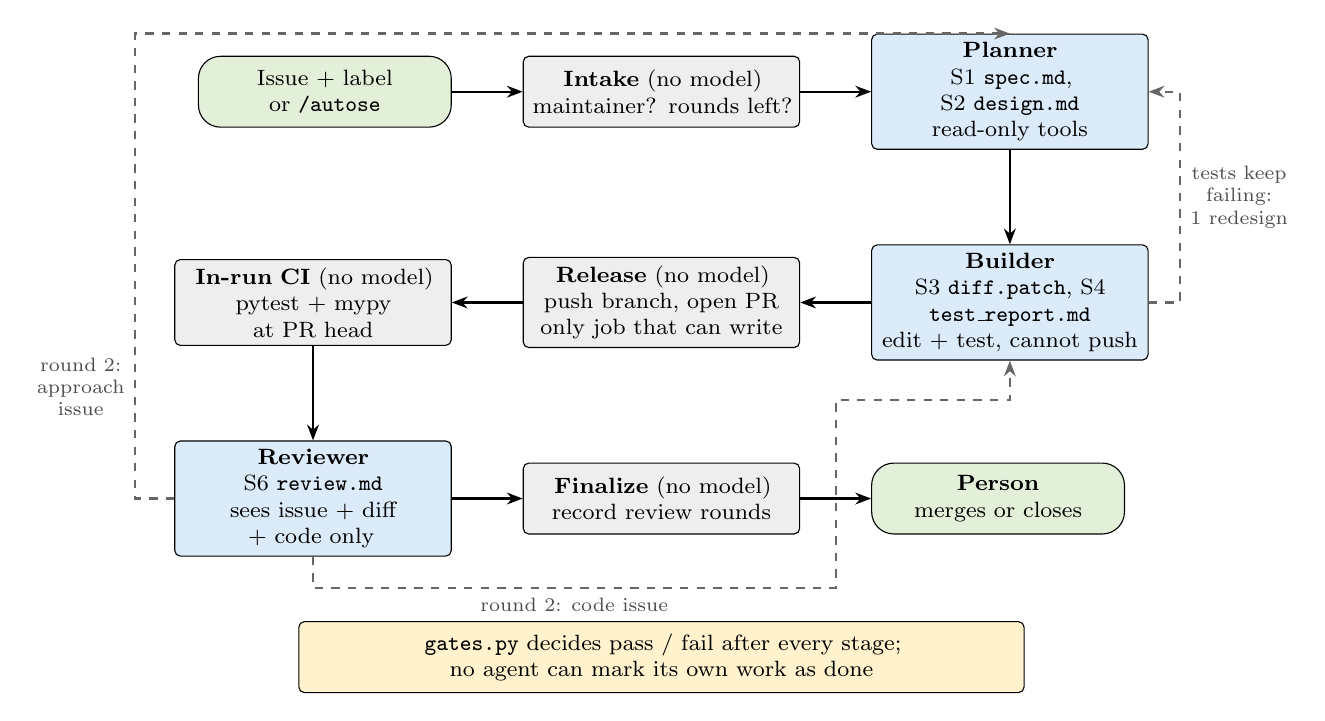
\begin{tikzpicture}[node distance=5mm and 9mm]
  \node[humanbox] (issue) {Issue + label\\or \code{/autose}};
  \node[scriptbox, right=of issue] (intake) {\textbf{Intake} (no model)\\maintainer? rounds left?};
  \node[agentbox, right=of intake] (plan) {\textbf{Planner}\\S1 \code{spec.md}, S2 \code{design.md}\\read-only tools};
  \node[agentbox, below=12mm of plan] (build) {\textbf{Builder}\\S3 \code{diff.patch}, S4 \code{test\_report.md}\\edit + test, cannot push};
  \node[scriptbox, left=of build] (release) {\textbf{Release} (no model)\\push branch, open PR\\only job that can write};
  \node[scriptbox, left=of release] (ci) {\textbf{In-run CI} (no model)\\pytest + mypy at PR head};
  \node[agentbox, below=12mm of ci] (review) {\textbf{Reviewer}\\S6 \code{review.md}\\sees issue + diff + code only};
  \node[scriptbox, right=of review] (fin) {\textbf{Finalize} (no model)\\record review rounds};
  \node[humanbox, right=of fin] (person) {\textbf{Person}\\merges or closes};
  \node[gatebox, text width=90mm, below=11mm of fin] (gates) {\code{gates.py} decides pass / fail after every stage; no agent can mark its own work as done};

  \draw[arr] (issue) -- (intake);
  \draw[arr] (intake) -- (plan);
  \draw[arr] (plan) -- (build);
  \draw[arr] (build) -- (release);
  \draw[arr] (release) -- (ci);
  \draw[arr] (ci) -- (review);
  \draw[arr] (review) -- (fin);
  \draw[arr] (fin) -- (person);
  \draw[back] (build.east) -- ++(4mm,0) |- node[note, pos=0.25, right] {tests keep\\failing:\\1 redesign} (plan.east);
  \coordinate (mx) at ($(fin.east)!0.5!(person.west)$);
  \coordinate (bs) at ($(build.south)+(0,-5mm)$);
  \draw[back] (review.south) -- ++(0,-4mm) -| node[note, pos=0.25, below] {round 2: code issue} (mx |- bs) -| (build.south);
  \draw[back] (review.west) -- ++(-5mm,0) |- node[note, pos=0.12, left] {round 2:\\approach\\issue} (plan.north);
\end{tikzpicture}
\caption{Component view. Blue boxes are agents, grey boxes are scripts without a model, and dashed
arrows are the bounded loops back. The full view with tools and permissions is in
\code{architecture/views/component-view.md}.}
\label{fig:component}
\end{figure}

\begin{table}[h]
\centering\footnotesize
\caption{Stage map: agent, job, artifact and check for each stage.}
\label{tab:stagemap}
\begin{tabularx}{\textwidth}{@{}l l l l L@{}}
\toprule
Stage & Agent / component & Job (permissions) & Artifact & Check before moving on (\code{gates.py}) \\
\midrule
1 Requirements & Planner + testability judge & \code{plan} (read, issues) & \code{spec.md} & 2--6 Given/When/Then criteria, no vague words, every criterion judged testable \\
2 Design & Planner (uses \code{ARCHITECTURE.md}) & \code{plan} & \code{design.md} & named files exist, named functions exist (AST check), paths in allowlist \\
3 Implementation & Builder & \code{build} (read only) & \code{diff.patch} & non-empty, allowed paths only, \code{git apply} works, build passes \\
4 Testing & Builder & \code{build} & \code{test\_report.md} & full suite passes, each criterion maps to a passing \emph{new} test, no new skips \\
5 Release & Script, then in-run CI & \code{release} (write), \code{ci} & \code{pr.md} + PR & PR open in the fork on \code{autose/issue-N}, CI status success \\
6 Review & Reviewer & \code{review} (read, PR) & \code{review.md} & valid verdict, four audit dimensions, tests were run, defects cite file and line \\
\bottomrule
\end{tabularx}
\end{table}

\textbf{Bounds.} In each round the Builder has at most two cycles of three attempts, with one design
revision between them, and there are at most two review rounds. Every stage also has a turn limit, a
token limit, a cost limit and a job timeout. Each job checks out the workflow code from \code{master}
into a separate folder from the code being changed, so a pull request cannot change the rules it is
checked against.

\textbf{Models.} My first five runs used the Gemini free tier: \code{gemini-3.5-flash-lite} for
planning, and \code{gemini-3.5-flash} and \code{gemini-3.6-flash} for building and reviewing, with other
Gemini models as fallbacks when one ran out of quota. All my later runs used DeepSeek:
\code{deepseek-flash} (DeepSeek V4.1 Flash) for the Planner and Builder and, at first,
\code{deepseek-v4-pro} (DeepSeek V4 Pro) for the Reviewer. In the end I put every role
on \code{deepseek-flash} to keep it simple and cheap, and used V4 Pro again only in experiment~A.

\begin{figure}[h]
\centering
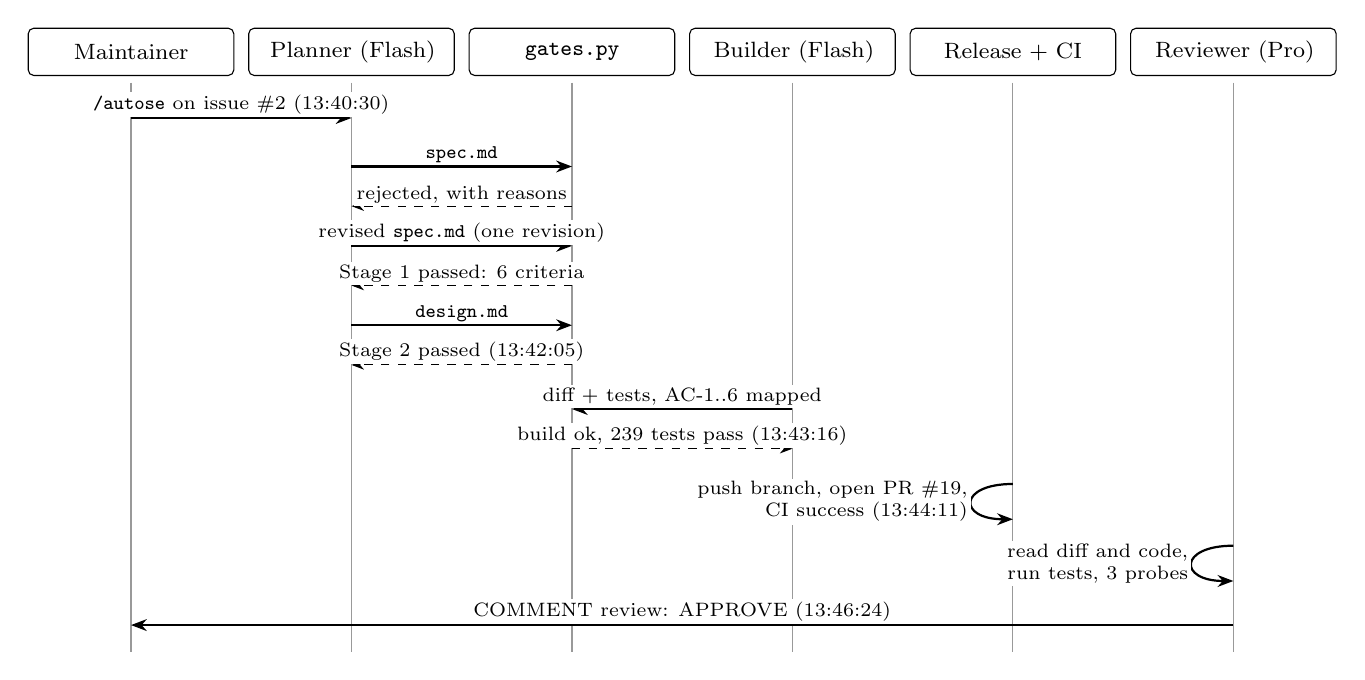
\begin{tikzpicture}[x=28mm, y=-5.6mm, font=\scriptsize]
  % lanes
  \foreach \x/\name in {0/Maintainer, 1/Planner (Flash), 2/\code{gates.py}, 3/Builder (Flash), 4/Release + CI, 5/Reviewer (Pro)} {
    \node[box, fill=white, text width=24mm, minimum height=6mm] at (\x,0) {\name};
    \draw[black!40] (\x,0.7) -- (\x,13.6);
  }
  \newcommand{\msg}[4]{\draw[arr] (#1,#3) -- node[above, font=\scriptsize, align=center, fill=white, inner sep=1pt] {#4} (#2,#3);}
  \newcommand{\ret}[4]{\draw[-{Stealth[length=1.6mm]}, dashed] (#1,#3) -- node[above, font=\scriptsize, align=center, fill=white, inner sep=1pt] {#4} (#2,#3);}
  \msg{0}{1}{1.5}{\code{/autose} on issue \#2 (13:40:30)}
  \msg{1}{2}{2.6}{\code{spec.md}}
  \ret{2}{1}{3.5}{rejected, with reasons}
  \msg{1}{2}{4.4}{revised \code{spec.md} (one revision)}
  \ret{2}{1}{5.3}{Stage 1 passed: 6 criteria}
  \msg{1}{2}{6.2}{\code{design.md}}
  \ret{2}{1}{7.1}{Stage 2 passed (13:42:05)}
  \msg{3}{2}{8.1}{diff + tests, AC-1..6 mapped}
  \ret{2}{3}{9.0}{build ok, 239 tests pass (13:43:16)}
  \draw[arr] (4,9.8) to[out=180,in=180,looseness=4] node[left, font=\scriptsize, align=right, fill=white, inner sep=1pt] {push branch, open PR \#19,\\CI success (13:44:11)} (4,10.6);
  \draw[arr] (5,11.2) to[out=180,in=180,looseness=4] node[left, font=\scriptsize, align=right, fill=white, inner sep=1pt] {read diff and code,\\run tests, 3 probes} (5,12.0);
  \msg{5}{0}{13.0}{COMMENT review: APPROVE (13:46:24)}
\end{tikzpicture}
\caption{Sequence view of a real run on DeepSeek: issue \#2, run 45186252584. The whole run took
6~min~13~s and cost about \$0.089 (Planner 15 model calls, Builder 20, Reviewer 11). The version with
numbers per stage is in \code{architecture/views/sequence-view.md}.}
\label{fig:sequence}
\end{figure}

%==================================================================================================
\section{Design Decisions}

I wrote thirteen architecture decision records (ADRs) in the Nygard format; they are in
\code{architecture/decisions/}. I committed ADR-001 to ADR-010 before writing any agent code. I added
ADR-011 to ADR-013 later, when real runs showed me that an earlier decision was wrong, and I kept the
old ADRs and marked them as superseded.

\begin{table}[h]
\centering\scriptsize
\caption{Summary of all ADRs.}
\label{tab:adrs}
\begin{tabularx}{\textwidth}{@{}l p{18mm} L L L p{15mm}@{}}
\toprule
ADR & Decision & Option chosen & Main option rejected & Main reason & Status \\
\midrule
001 & D1 Splitting the work & 3 agents (Planner 1--2, Builder 3--4, Reviewer 6) + scripted release & one agent, or one per stage & planning reads, building writes, release pushes, review judges; fewer cold starts than six agents & Accepted \\
002 & D2 Control flow & fixed state machine in an unrolled multi-job DAG & LLM orchestrator choosing the next step & guaranteed termination, no tokens spent on routing & Accepted \\
003 & D3 Hand-offs & small structured artifacts; reviewer gets only issue, diff and code & passing transcripts on & less context, reviewer not anchored, untrusted text kept from the Builder & Accepted \\
004 & D4 State & Actions artifacts in a run; branch + bot-written comment across runs & committing \code{.autose/} files to the PR & clean PR diffs, reviewer cannot see upstream files, safe restarts & Accepted \\
005 & D5 Tools & small tool set per role + per-job token permissions & GitHub MCP server in every job & least privilege enforced by GitHub, small tool schemas & Accepted \\
006 & D6 Models & Claude Sonnet/Haiku + GPT-5 reviewer & one model everywhere & cost tiers, reviewer from another family & Superseded by 011 \\
007 & D7 Checks & plain-code gates; model judge only for testability & LLM judge at every stage & Stages 2--6 have objective checks & Partly superseded by 012 \\
008 & D8 Reviewer independence & own job, no upstream artifacts, other model, skeptical rubric that needs evidence & review in the Builder's job & prevent rubber-stamp approvals & Accepted \\
009 & D9 Safety & timeouts, caps, issue read via env only, path allowlist, no secrets in test runs & default timeouts, prompt-only safety & bounded cost, no injection path to secrets or workflows & Accepted \\
010 & D10 Triggers & label or maintainer comment; one lock per issue & trigger on every new issue & outsiders cannot spend budget, no branch races & Accepted \\
011 & D6 (2nd) & Gemini free tier, fallback model lists & paying for Claude & no paid API access & Superseded by 013 \\
012 & D7 (2nd) & Planner gets one revision with the gate's reasons & halt on the first failed check & a run stopped on one fixable sentence & Accepted \\
013 & D6 (3rd) & DeepSeek (\code{deepseek-flash} for every role) & waiting out Gemini quotas & 4 of 5 Gemini runs failed on overload or quota & Accepted \\
\bottomrule
\end{tabularx}
\end{table}

\subsection*{The three most important decisions}

\textbf{Plain code decides, not the agents (ADR-007, revised by ADR-012).} A stage hands over only when
\code{gates.py} says it has passed. The design check parses the plan and confirms that every function
it names exists in the code. The test check runs the full suite and confirms that each acceptance
criterion maps to a new test that passed. In my runs these checks caught real mistakes: a criterion stating that an
existing test ``continues to function correctly'' was rejected as untestable, and a Builder that mapped a
criterion to a test that did not exist was sent back. They also showed me my own bugs first,
such as a parser that read only the first line of a criterion written over two lines, so I kept the
gates small and covered them with unit tests (38 in total). The one rule I changed was halting on the
first failure. Run 45172879048 stopped after one minute because of one vague sentence that the
checker had already explained. So in ADR-012 I gave the Planner exactly one revision using the
checker's reasons. In the run in Figure~\ref{fig:sequence}, this revision is what let Stage~1 pass.

\textbf{Reviewer independence through structure (ADR-008, ADR-003).} I did not want independence to
depend on the prompt, so I built it into the structure. The Reviewer runs in its own job with a read-only checkout of the pull request and never
downloads the specification, the design or any notes from the other agents. It receives what a human
reviewer would receive: the issue, the diff and the code, and it may run the tests and its own short
Python probes. An approval must be supported by evidence: the gate rejects a review that did not run the
tests or skipped one of the four audit dimensions, and every blocking defect must cite a file and a line.
GitHub does not allow a bot to approve its own pull request, so the Reviewer posts a comment with its
verdict, and only a person can approve and merge. Because the Reviewer reads the issue rather than the
specification, it judges what the user asked for, not the Planner's interpretation of it.

\textbf{The model decision, made three times (ADR-006, 011, 013).} I designed the workflow for Claude,
but then found I had no paid API access. I moved it to the Gemini free tier, which needed new handling:
waiting for the delay the server requests, stopping at once when the daily quota is used up, and a list
of fallback models for each role. Each of my five Gemini runs on issue \#3 showed me something to fix,
but four of them failed on overload or quota, and the one that finished spent about 45 minutes in the
Builder. After I moved to DeepSeek, the same pipeline completed an issue in about six minutes for
under ten cents (Figure~\ref{fig:providers}). The structure did not change across the three providers;
only the model client and the limits did. DeepSeek needed 40 Builder turns instead of 20, because it
tends to take one small step per turn.

\begin{figure}[h]
\centering
\begin{tikzpicture}[font=\footnotesize]
  \node[box, fill=script, text width=36mm] (c) {\textbf{Claude} (ADR-006)\\designed for, never run\\no paid API access};
  \node[box, fill=gate, text width=34mm, right=16mm of c] (g) {\textbf{Gemini free tier} (ADR-011)\\5 runs, 0 completed\\overload and daily quota\\1 PR built in ${\approx}$45 min};
  \node[box, fill=human, text width=34mm, right=16mm of g] (d) {\textbf{DeepSeek} (ADR-013)\\9 full runs, 4 completed\\after harness fixes\\issue \#2 in 6 min, \$0.09};
  \draw[arr] (c) -- node[above, note] {no access} (g);
  \draw[arr] (g) -- node[above, note] {quota} (d);
\end{tikzpicture}
\caption{How the model decision changed during the project.}
\label{fig:providers}
\end{figure}

%==================================================================================================
\section{Decision Experiments}

I tested two decisions on five seeded pull requests (\code{experiment/seeded\_prs/}). Four contain a
bug that I planted on purpose and one is a correct fix. All five pass TinyDB's own test suite, so the
bugs cannot be found just by running the tests. I kept the answer key outside the repository until every
review had finished. All experiment reviews ran on DeepSeek.

\begin{itemize}
\item \textbf{Experiment A} tests the reviewer model (ADR-008, ADR-013): the same skeptical prompt on
DeepSeek V4 Pro instead of V4.1 Flash.
\item \textbf{Experiment B} tests the skeptical prompt (ADR-008): V4.1 Flash with a plain prompt that does
not tell the Reviewer to assume the change is wrong and does not ask for probes.
\end{itemize}

\begin{table}[h]
\centering\footnotesize
\caption{Reviewer verdicts on the seeded pull requests. ``Changes'' means REQUEST\_CHANGES.}
\label{tab:experiments}
\begin{tabularx}{\textwidth}{@{}L l l l@{}}
\toprule
Seed and planted problem & Baseline: Flash, skeptical & A: Pro, skeptical & B: Flash, plain \\
\midrule
S1: fragment queries made uncacheable (wrong approach) & changes, to implementation & changes, to \textbf{design} & changes, to implementation \\
S2: duplicate ids fixed in \code{remove()} only & changes & changes & changes (after a format repair) \\
S3: limit applied before caching & changes & changes & changes \\
S4: rename crashes on documents without the field & changes & changes & changes \\
S5: correct fix & approve & approve & approve \\
\midrule
\textbf{Bugs caught / false alarms} & \textbf{4/4, 0} & \textbf{4/4, 0} & \textbf{4/4, 0} \\
Probes before approving S5 & 7 (19 turns) & 3 (14 turns) & 3 (12 turns) \\
Tokens / estimated cost, all five & 713K / \$0.059 & 635K / \$0.196 & 339K / \$0.038 \\
\bottomrule
\end{tabularx}
\end{table}

\begin{figure}[h]
\centering
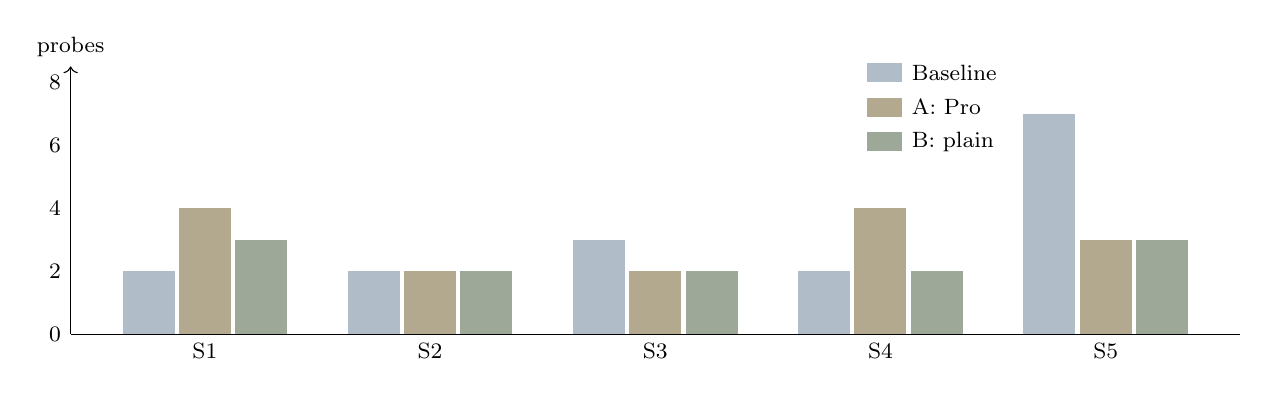
\begin{tikzpicture}[font=\footnotesize, x=11mm, y=4mm]
  \draw[->] (0,0) -- (0,8.5) node[above] {probes};
  \draw (0,0) -- (13.5,0);
  \foreach \v in {0,2,4,6,8} \node[left] at (0,\v) {\v};
  % groups: S1..S5, three bars each
  \foreach \i/\s/\b/\a/\p in {0/S1/2/4/3, 1/S2/2/2/2, 2/S3/3/2/2, 3/S4/2/4/2, 4/S5/7/3/3} {
    \pgfmathsetmacro{\xo}{0.6+\i*2.6}
    \fill[agent!80!black] (\xo,0) rectangle ++(0.6,\b);
    \fill[gate!70!black] (\xo+0.65,0) rectangle ++(0.6,\a);
    \fill[human!70!black] (\xo+1.3,0) rectangle ++(0.6,\p);
    \node[below] at (\xo+0.95,0) {\s};
  }
  \fill[agent!80!black] (9.2,8.0) rectangle ++(0.4,0.6); \node[right] at (9.6,8.3) {Baseline};
  \fill[gate!70!black] (9.2,6.9) rectangle ++(0.4,0.6); \node[right] at (9.6,7.2) {A: Pro};
  \fill[human!70!black] (9.2,5.8) rectangle ++(0.4,0.6); \node[right] at (9.6,6.1) {B: plain};
\end{tikzpicture}
\caption{Edge-case probes run by the Reviewer on each seed. The skeptical Flash reviewer probed the
clean seed S5 most before approving it.}
\label{fig:probes}
\end{figure}

\textbf{Findings.} Neither change altered a single verdict. Every setup caught all four bugs and
approved the clean pull request, each time citing the file and line and usually reproducing the bug
with a probe. For both ADRs as I wrote them, this is a negative result: on these seeds, the structural
controls (own job, no upstream artifacts, an evidence-based rubric) appear to do most of the work. Two
differences were real. With the skeptical prompt, the Reviewer checked much more carefully before
approving (seven probes on the clean pull request instead of three; Figure~\ref{fig:probes}), which is
the behaviour ADR-008 aimed for. Only V4 Pro recognised that the problem in S1 was the approach rather
than the code and routed it to the design stage. In a second round, this decides whether the change is
re-planned or only patched. V4 Pro cost about 3.3 times as much as the baseline.

\textbf{What I changed.} I kept the Flash reviewer with the skeptical prompt as the default. The
experiment also exposed two bugs in my harness: the \code{model=} option did not accept DeepSeek model names,
and a review returned in the wrong JSON shape caused the job to crash. ADR-007 already allowed one
format-repair pass, so I gave the Reviewer one chance to resubmit. If I continued, I would use V4 Pro
only to confirm the routing of a REQUEST\_CHANGES verdict.

%==================================================================================================
\section{Results}

All five issues passed through every stage. Each ended with a pull request that the Reviewer approved
and that passes my hidden acceptance tests, which the agents never saw (Table~\ref{tab:results}).
Pull request \#16 was built on the Gemini free tier, but the Gemini reviewer had no quota left, so I
had it reviewed later on DeepSeek V4 Pro. The other four were built and reviewed on DeepSeek.

\begin{table}[h]
\centering\footnotesize
\caption{Outcome for each issue.}
\label{tab:results}
\begin{tabularx}{\textwidth}{@{}l l L l l@{}}
\toprule
Issue (type) & PR & Change made by the agents & Built on & Hidden tests \\
\midrule
\#2 \code{remove()} with duplicate ids (bug) & \#19 & duplicate ids removed in \code{update()} and \code{remove()}; 6 tests & DeepSeek & 3/3 \\
\#3 \code{fragment()} on two fields (bug) & \#16 & field path added to the query's cache key & Gemini & 3/3 \\
\#4 rename operation (feature) & \#23 & new \code{operations.rename}; documents without the field are left unchanged & DeepSeek & 3/3 \\
\#5 search limit (feature) & \#20 & optional \code{limit}; the cache still holds the full result & DeepSeek & 4/4 \\
\#6 dates (vague) & \#28 & dates tagged in the JSON file and converted back on read & DeepSeek & 3/3 \\
\bottomrule
\end{tabularx}
\end{table}

\begin{figure}[h]
\centering
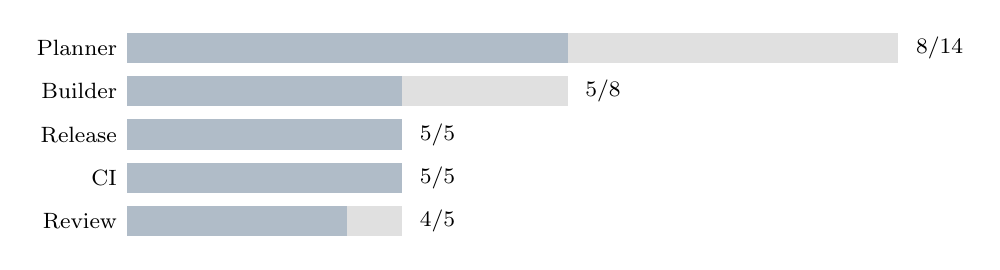
\begin{tikzpicture}[font=\footnotesize, x=1mm, y=5.5mm]
  \foreach \i/\name/\pass/\ran in {0/Planner/8/14, 1/Builder/5/8, 2/Release/5/5, 3/CI/5/5, 4/Review/4/5} {
    \node[left] at (0,-\i) {\name};
    \fill[black!12] (0,-\i-0.35) rectangle ++(\ran*7,0.7);
    \fill[agent!80!black] (0,-\i-0.35) rectangle ++(\pass*7,0.7);
    \node[right] at (\ran*7+1,-\i) {\pass/\ran};
  }
\end{tikzpicture}
\caption{Pass rate per stage over all 14 full runs, including debugging runs. Dark: passed; light:
reached the stage.}
\label{fig:passrate}
\end{figure}

\textbf{Pass rates.} Figure~\ref{fig:passrate} shows the pass rate per stage over all 14 full runs
(\code{results/results.csv}). On the Gemini free tier, none of the five runs completed; they failed on
overload and quota, and the single review that failed had no quota left. On DeepSeek, four of nine runs
completed. The other five stopped on problems in my harness (turn limits set for Claude, a judge answer that
was cut off, criteria written over several lines); I fixed each one and ran the issue again. All runs
together used about 5.9 million tokens and cost about \$0.85 on DeepSeek. The Gemini runs were free.

\textbf{What the Reviewer caught.} On the seeded pull requests it found all four planted bugs, each with
a probe, as well as real problems that I had not planted: in S3, \code{limit=0} permanently caches an empty
result, and the crash in S4 leaves the data partly updated. It approved all five pull requests produced
by the agents, but still noted points for a person to check. On \#6 it found that a user document whose
only key is the reserved date tag would silently be converted into a date when read back.

\textbf{Where it was wrong.} The Flash reviewer routed S1 to implementation, although the approach was
the problem. On \#6, the reserved-key issue is arguably a real defect that it accepted as non-blocking.
It also noticed that my seeded tests had the word ``seeded'' in their names, a hint I did not intend
to give.

%==================================================================================================
\section{Hindsight}

The first decision I would change is the model decision (ADR-006). I chose models for their ability
and price, and only at the first run did I find out that I could not use them, and later that the Gemini
free tier was too slow and too limited for this work. If I started again, I would treat access, quotas
and model behaviour as design inputs and check them with a one-call test before writing any agent code
(I only added the ``check models'' workflow later). I would also make the provider and all limits plain
configuration from the start; I had to change the turn limits, timeouts and token caps twice because I
had set them for a model I never ran. Finally, I would give the Planner its one revision from the
beginning instead of halting, since the Builder already had retries.

%==================================================================================================
\section{Limitations and Threats to Validity}

\begin{itemize}
\item \textbf{Small sample.} Five issues and five seeded pull requests, with one run per experiment cell.
A 4/4 against 4/4 tie says little about cases where the setups would differ, and one different verdict
would change the picture.
\item \textbf{I wrote everything I measured with.} The issues, hidden tests, seeds and prompts are all
mine, so they may suit each other. The hidden tests for the vague issue accept more
than one reasonable answer, which also makes them easier to pass.
\item \textbf{The system changed while I measured it.} The results come from a harness that changed over
time (two providers in real runs and several fixes). The final setup, Flash for every role, reviewed
only two of the five issue pull requests; V4 Pro reviewed the other three.
\item \textbf{Round 2 was never exercised in a real run.} Every agent pull request was approved in round
1, so the path back to the Builder or Planner is covered only by unit tests.
\item \textbf{Same provider for Builder and Reviewer.} In the final setup they also use the same model, so
they may share blind spots. Only experiment~A used a different model.
\item \textbf{Safety gaps.} GitHub-hosted runners do not restrict network access, so code written by the
Builder can make outbound requests while tests run, although it has no secrets to send. The hidden tests
are now in the repository, so any later run could read them.
\end{itemize}

\vspace{2pt}
{\small\textbf{Use of AI tools.} I used Claude Code to help build the harness and to draft parts of the
documentation. I went through everything it produced, and the design decisions and the reasoning in
the ADRs are my own. Every run, pull request and review in this report is real and linked in
\code{results/runs.md}.}

\end{document}
